\documentclass[aspectratio=169]{beamer}
\usepackage[framemethod=tikz]{mdframed}
\usepackage{pgfplots}
\usepackage{tikz}
\usepackage{url}
\usepackage{xcolor}
\usepackage{qrcode}
\usepackage{xmpmulti}
\usetikzlibrary{shapes,arrows}
\hypersetup{pdfstartview={Fit}} % Fit the presentation to the window when first displayed
\usetheme{Frankfurt}
\pgfplotsset{compat=1.14}
\beamertemplatenavigationsymbolsempty{} % Remove Beamer navigation symbols
\nonstopmode{} % Keep making the file through errors
\usepackage[sfdefault]{sourcesanspro}
\usepackage[T1]{fontenc}

% http://danielfalster.com/blog/2013/06/18/a-nice-title-page-for-beamer-presentations/
\newmdenv[tikzsetting={draw=black,fill=white,fill opacity=0.7, line width=1pt},backgroundcolor=none,leftmargin=0,rightmargin=0,innertopmargin=5pt,skipbelow=\baselineskip,skipabove=\baselineskip]{TitleBox}

\title{Open House: \\ Open Source Home Automation}
\author[Swartz]{Tom~Swartz}
\institute{Central PA Open Source Conference}
\date{April 1 2023}
\subject{Computer Science}
\begin{document}

% Title Page
{\usebackgroundtemplate{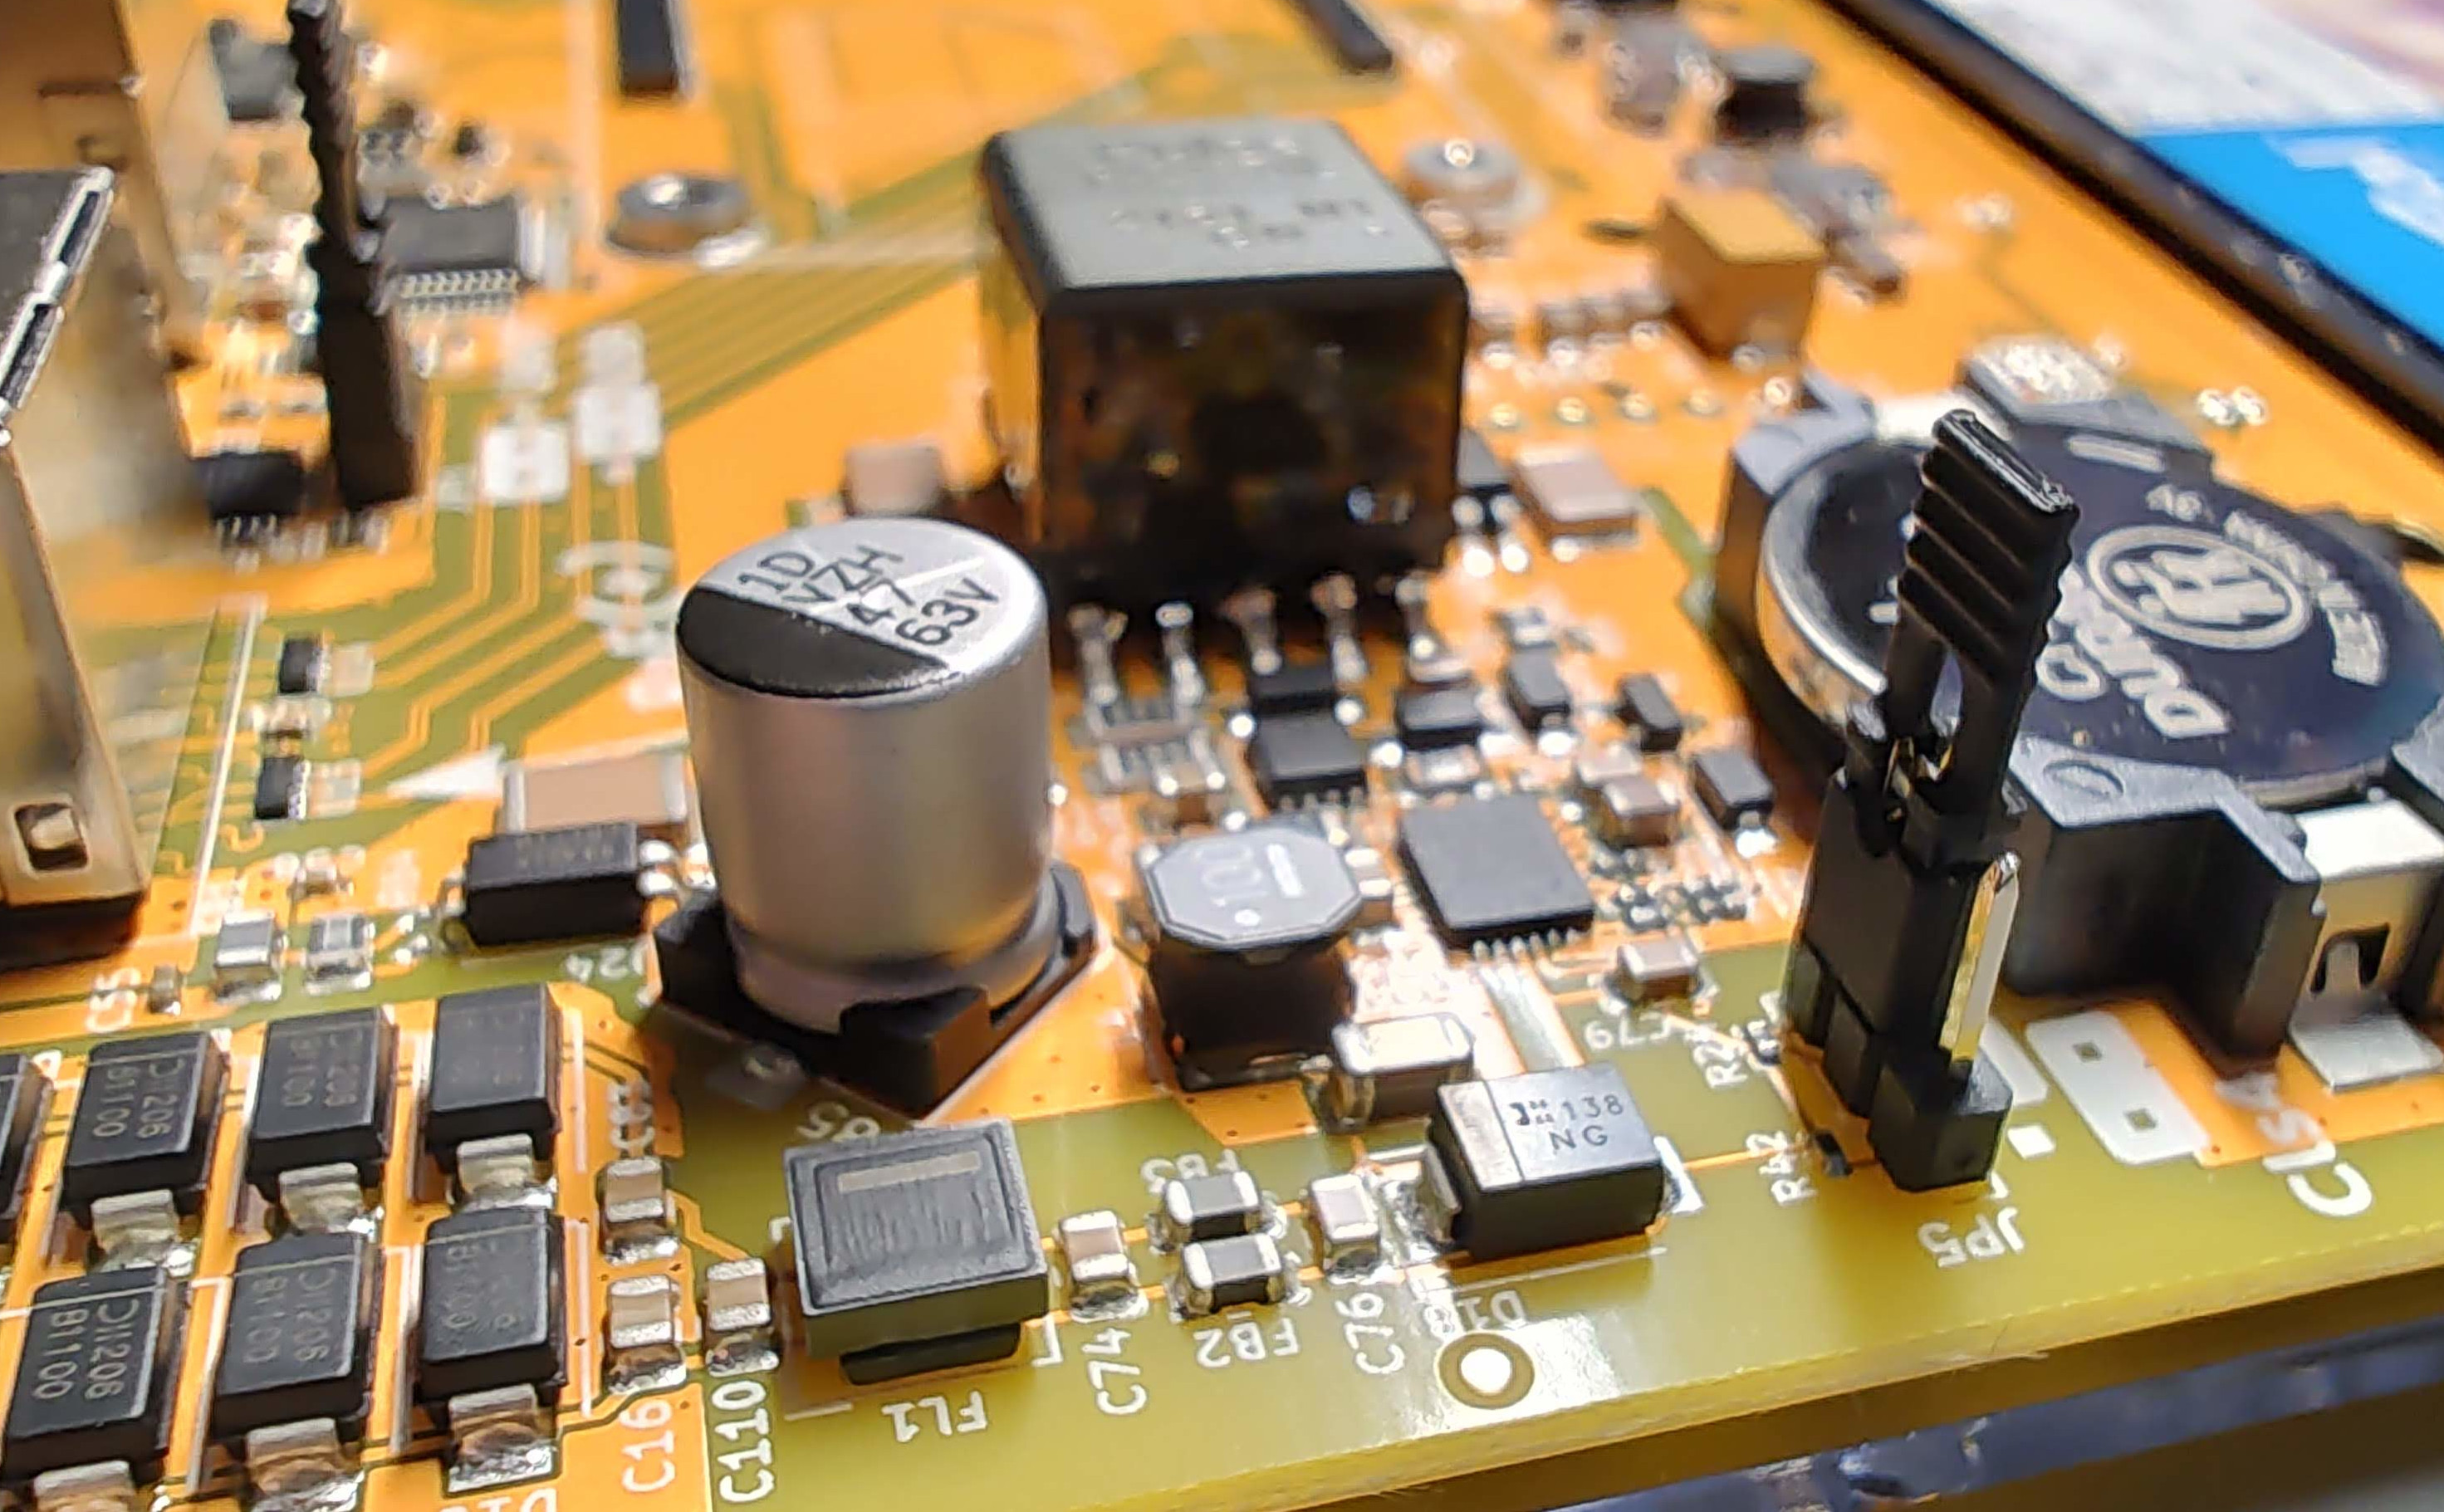
\includegraphics[width=1.00\paperwidth,keepaspectratio]{images/yellow-board.jpg}}
\begin{frame}[plain]
    \begin{TitleBox}
        \begin{center}
            {\color{red}\Large\inserttitle\color{black}}\\
        \end{center}
        \insertauthor{}\hfill\textbf{\insertinstitute{}}\hfill\insertdate{}\\
        {\footnotesize
        \href{https://hachyderm.io/@tswartz07}{@tswartz07@hachyderm.io}
        \hfill
        \href{mailto: tom@tswartz.net}{tom@tswartz.net}
        }
    \end{TitleBox}
    \vspace{15em}
\end{frame}}

\begin{frame}
  \frametitle{Who is this guy?}
  \framesubtitle{And what is he doing here?}
  \begin{columns}[]
    \begin{column}[T]{0.45\paperwidth}
      {\huge Tom Swartz}
      \vfill
      \begin{itemize}[<+->]
        \item{Crunchy Data \\ Associate Director of Support}
        \item{Hobbyist interests in `Big Data', IoT, RF Communications}
        \item{Prior CPOSC talks on RF comms/SDR \& homemade PCBs}
        \item{I've got some pretty specific hyperfixations}
      \end{itemize}
    \end{column}
    \begin{column}[T]{0.45\paperwidth}
      
\includegraphics[height=4cm,keepaspectratio]{images/logo.png}
    \end{column}
  \end{columns}
\end{frame}

\section{Home Assistant (and Friends)}
\begin{frame}
  \frametitle{Summary}
  We'll be reviewing the following topics, and how they relate to Home Automation
  \begin{enumerate}
    \item{Home Assistant}
    \item{ESPHome}
    \item{Building your own Sensors}
  \end{enumerate}
\end{frame}

\subsection{Home Assistant}
\frame{\subsectionpage}

\begin{frame}[fragile]
  \frametitle{Why Home Assistant?}
  \begin{columns}[]
    \begin{column}[T]{0.45\paperwidth}
      \begin{itemize}%[<+->]
        \item{There are a million apps for every `Smart' thing (sometimes multiple for the same item!)}
        \item{A practical application for consolidating software, apps, and tool-sets that many people already use}
        \item{Needs for better usability, security, and maintenance}
        \item{A solid use case for HomeLab equipment, for nerd cred}
        \item{It's Open Source!}
     \end{itemize}
    \end{column}
    \begin{column}[T]{0.45\paperwidth}
      
\includegraphics[height=4cm,keepaspectratio]{images/standards.png}
    \end{column}
  \end{columns}
\end{frame}

% Install Methods
\begin{frame}[fragile]
  \frametitle{Installation Methods}
  \begin{columns}[]
    \begin{column}[T]{0.45\paperwidth}
      \begin{enumerate}%[<+->]
        \item{Home Assistant Yellow}
        \item{Docker Container}
        \item{Dedicated Raspberry Pi \tiny{(Good luck finding one!)}}
        \item{Running as a background app on other hosts/servers}
      \end{enumerate}
      \emph{Worth noting that certain install methods lack certain features (such as third party add-ons)}
    \end{column}
    \begin{column}[T]{0.45\paperwidth}
      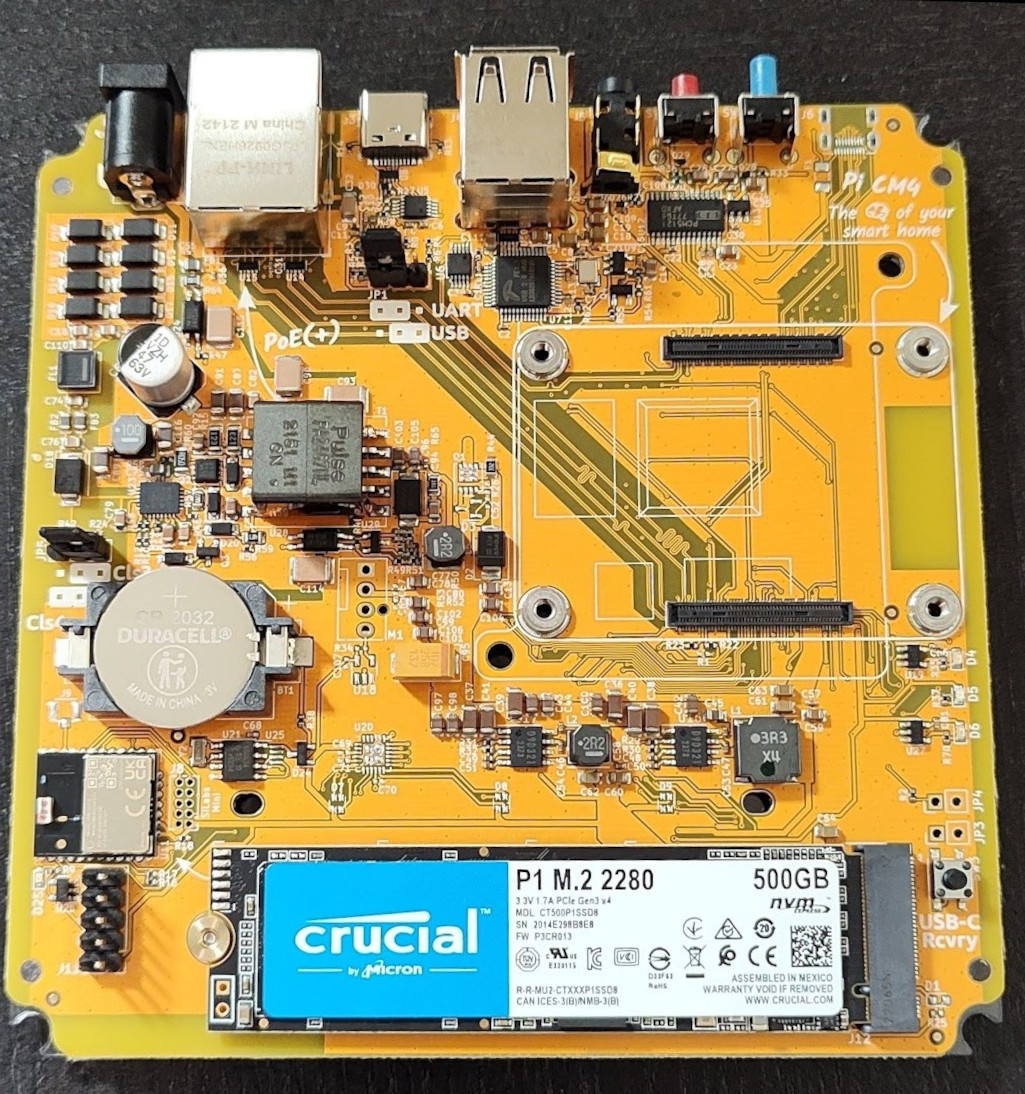
\includegraphics[height=6cm,keepaspectratio]{images/yellow.jpg}
    \end{column}
  \end{columns}
\end{frame}

\subsection{Components and Overview}
\begin{frame}[fragile]
  \frametitle{Components and Overview}
  Home Assistant is made of several parts:
  \begin{enumerate}%[<+->]
    \item{Dashboards}
    \item{Integrations}
    \item{Devices and Entities}
    \item{Automations}
  \end{enumerate}
\end{frame}

% Dashboards
\begin{frame}[fragile]
  \frametitle{Dashboards}
  Home Assistant's way of showing what's happening
  \vfill
  \begin{columns}[]
    \begin{column}[T]{0.45\paperwidth}
      \begin{enumerate}%[<+->]
        \item{Per-User Dashboards}
        \item{Show live and historical data}
      \end{enumerate}
      \emph{lorem ipsum}
    \end{column}
    \begin{column}[T]{0.45\paperwidth}
      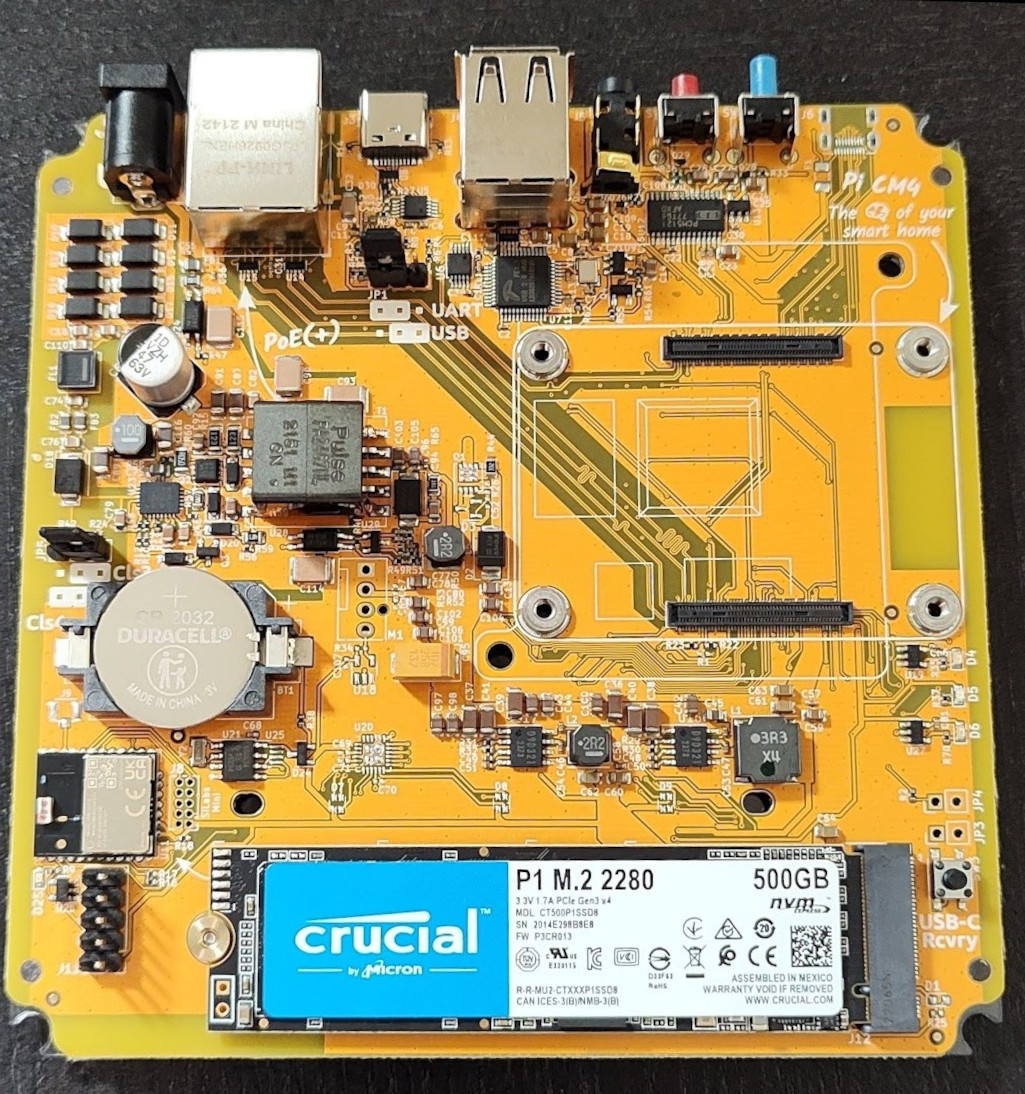
\includegraphics[height=6cm,keepaspectratio]{images/yellow.jpg}
    \end{column}
  \end{columns}
\end{frame}
% Integrations
\begin{frame}[fragile]
  \frametitle{Integrations}
  Arguably, the thing that makes Home Assistant so lucrative
  \vfill
  \begin{columns}[]
    \begin{column}[T]{0.45\paperwidth}
      \begin{enumerate}%[<+->]
        \item{All devices are community-driven}
        \item{2424+ total integrations supported}
        \item{Everything from 3D Printers to Vacuum cleaners}
      \end{enumerate}
    \end{column}
    \begin{column}[T]{0.45\paperwidth}
      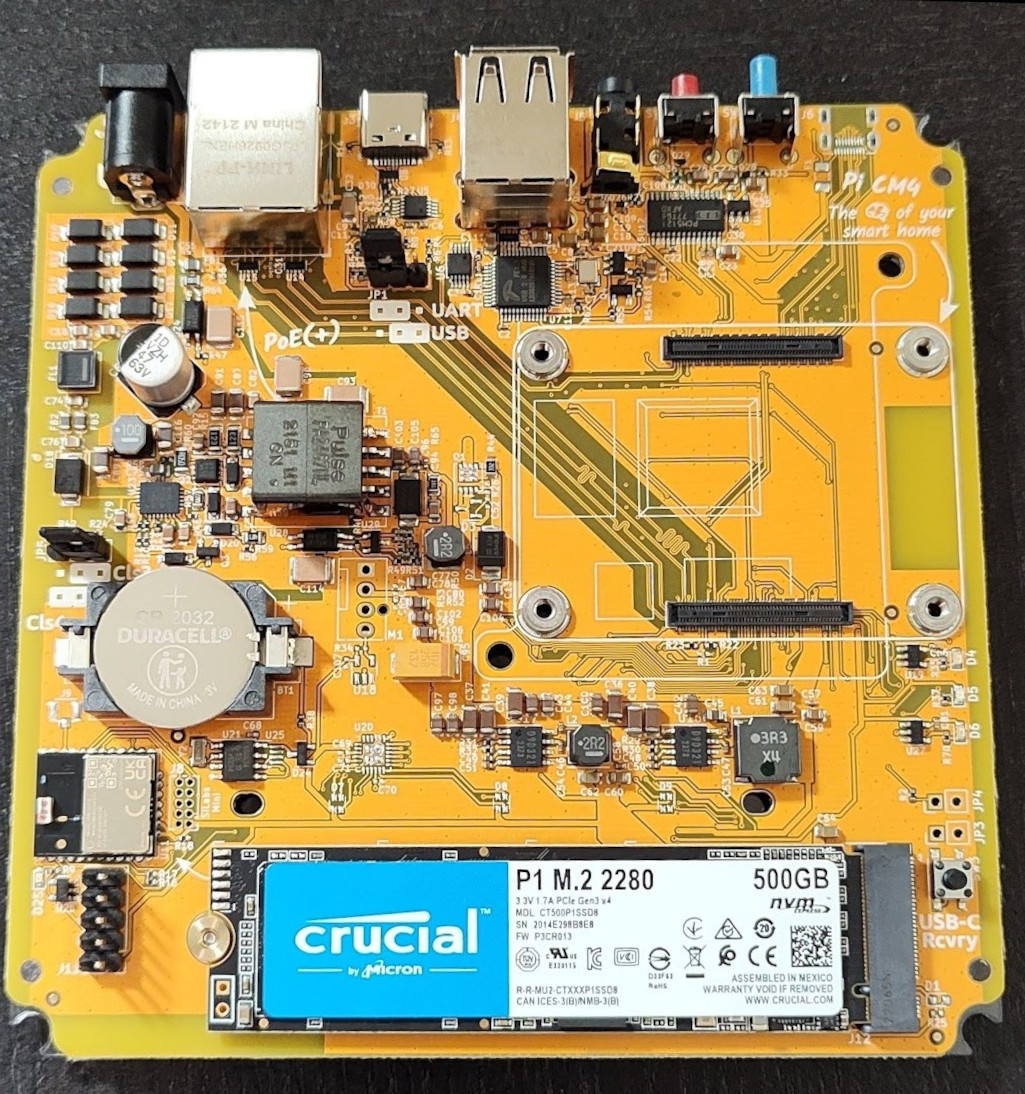
\includegraphics[height=6cm,keepaspectratio]{images/yellow.jpg}
    \end{column}
  \end{columns}
\end{frame}
\begin{frame}[fragile]
  \frametitle{Devices and Entities}
  The nuts and bolts of Home Assistant
  \vfill
  \begin{columns}[]
    \begin{column}[T]{0.45\paperwidth}
      \begin{description}%[<+->]
        \item[Devices]{A physical (or logical) group of sensors and inputs. For example, a motion sensor is a device}
        \item[Entities]{Any type of `data point' for a Device. For example, a motion sensor's \emph{Entities} can be: `Motion Status', `Battery Level', `Light Level'}
      \end{description}
    \end{column}
    \begin{column}[T]{0.45\paperwidth}
      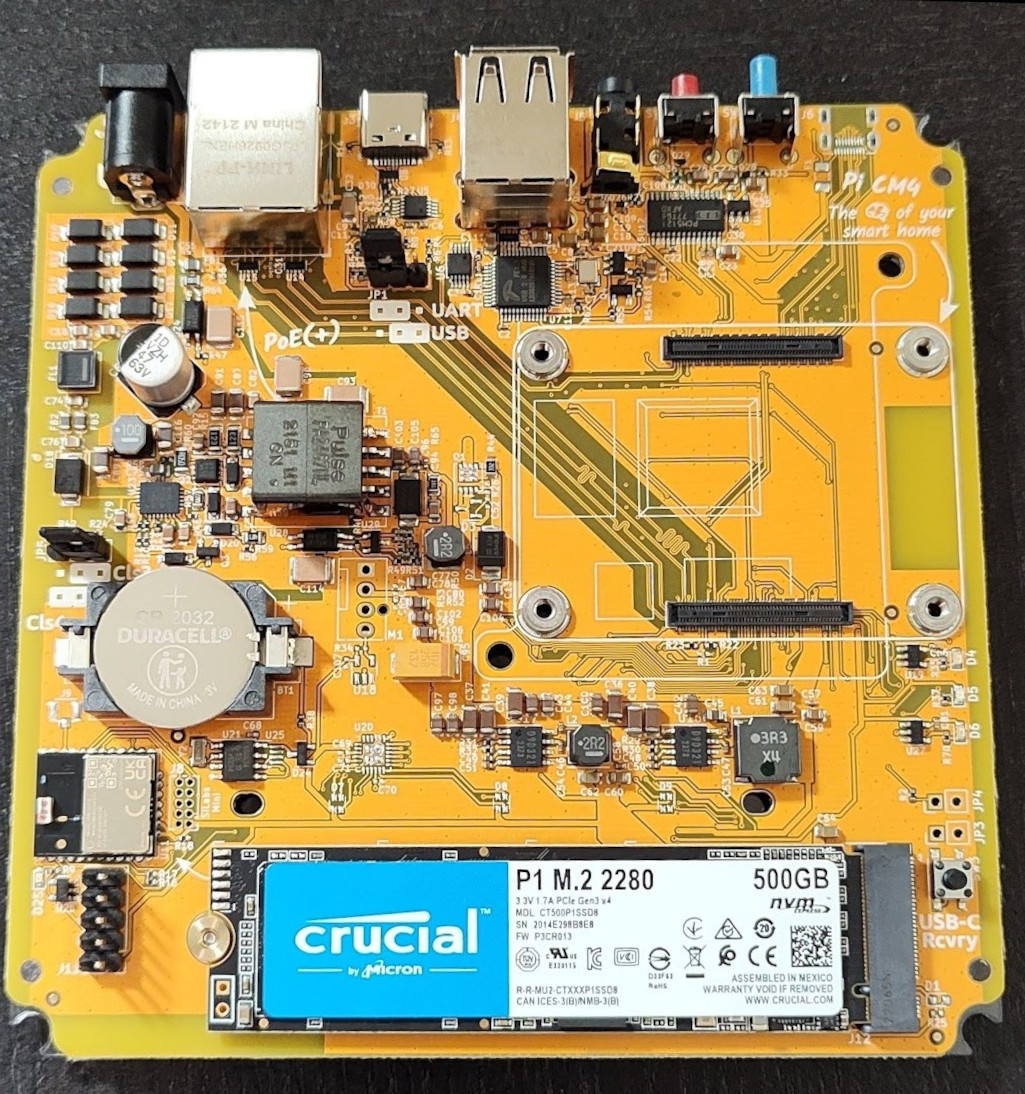
\includegraphics[height=6cm,keepaspectratio]{images/yellow.jpg}
    \end{column}
  \end{columns}
\end{frame}
\begin{frame}[fragile]
  \frametitle{Automations}
  Home Assistant's key features are Automations
  \vfill
  \begin{description}%[<+->]
    \item[Trigger]{Actions which will start the Automation action}
    \item[Conditions]{Optional conditions which limit when/where/how the automation will run}
    \item[Actions]{Items to perform if conditions are met}
  \end{description}
  \vfill
  It's kind of like $cron$, but for Internet of Things!
\end{frame}
\begin{frame}[fragile]
  \frametitle{Example Automations}
  Home Assistant performs Automations which allow for endless possibilities, but here are some examples:
  \vfill
  \begin{description}%[<+->]
    \item[Christmas Lights]{Turn on all of the Christmas lights 30 minutes before the sun sets}
    \item[Extra doorbell coverage]{Home Audio speakers announce if the doorbell is ringing}
    \item[Never forget to close the garage]{Automatically close the garage doors if no one is home}
    \item[Fix a dark office]{Turn on office lamps if it gets cloudy/dark}
  \end{description}
\end{frame}
\begin{frame}[fragile]
  \frametitle{So that means\ldots}
  \begin{columns}[]
    \begin{column}[T]{0.45\paperwidth}
      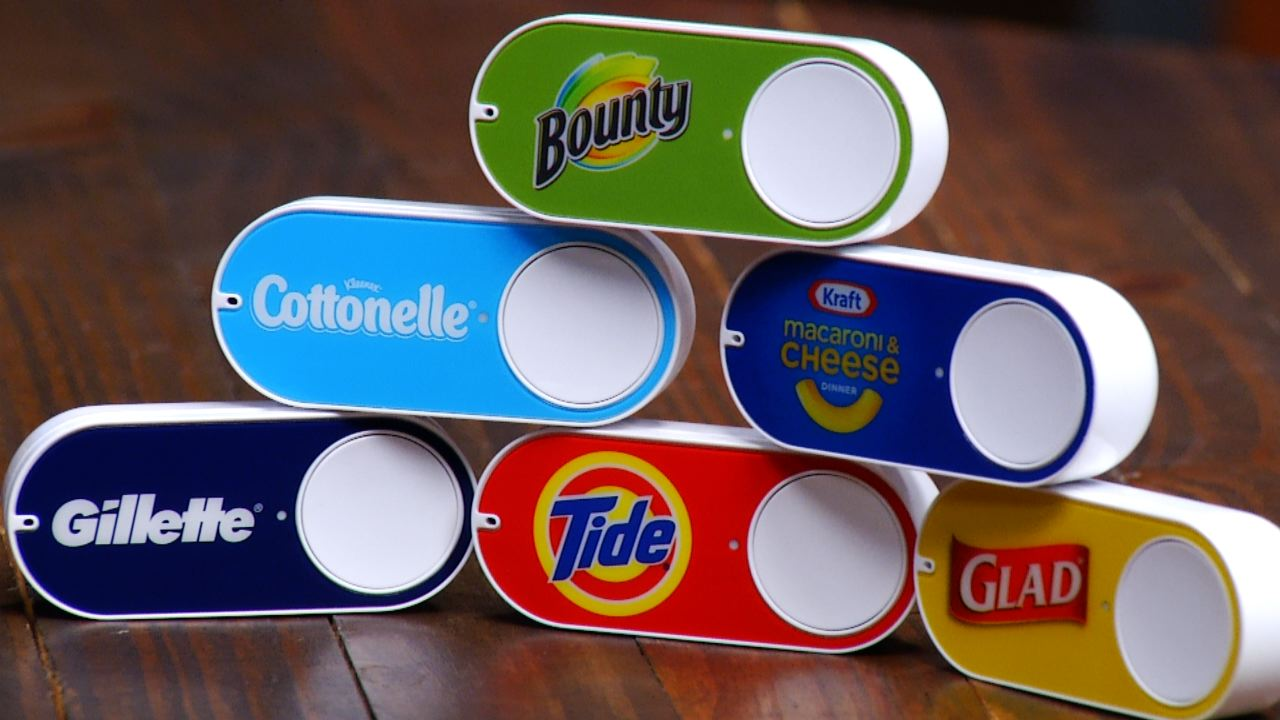
\includegraphics[width=0.4\paperwidth,keepaspectratio]{images/amazon-button.jpg}
    \end{column}
    \begin{column}[T]{0.45\paperwidth}
      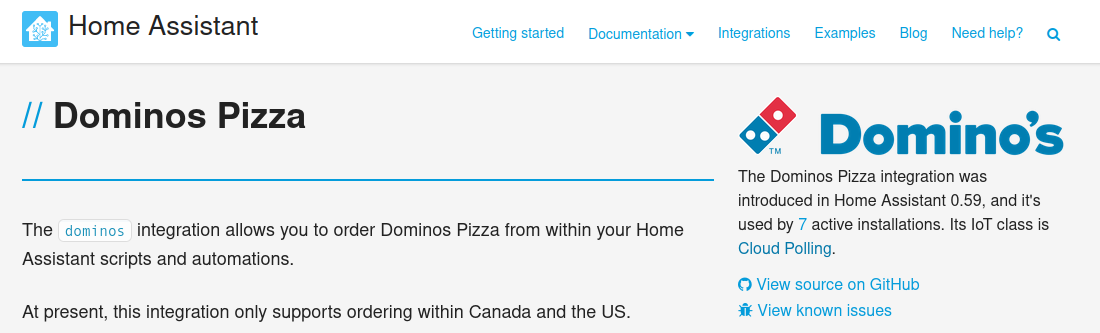
\includegraphics[width=0.45\paperwidth,keepaspectratio]{images/pizza.png}
    \end{column}
  \end{columns}
\end{frame}

\section{Security}
\frame{\sectionpage}
% Obvious need
\subsection{The Elephant in the Room}
\frame{\subsectionpage}
% How it compares; local control
\subsection{How does it compare?}
\frame{\subsectionpage}
\begin{frame}[fragile]
  \frametitle{Integration Classifications}
  Classifying the Internet of Things
  \vfill
  \begin{description}%[<+->]
    \item[Local Push]{Gold Standard, entirely local control directly from Home Assistant}
    \item[Local Poll]{Home Assistant direct read/write, but on-device updates may be delayed}
    \item[Cloud Push]{Integration of this device happens via the cloud and requires an active internet connection}
    \item[Cloud Poll]{Delayed integration of this device happens via the cloud and requires an active internet connection}
  \end{description}
\end{frame}

\section{Usage and Demo (Part 1)}
\subsection{Demo of Home-Assistant}
\frame{\subsectionpage}

\section{Custom Sensors}
\frame{\sectionpage}
\subsection{ESPHome}
\frame{\subsectionpage}
\begin{frame}[fragile]
  \frametitle{What is ESPHome?}
  \begin{columns}[]
    \begin{column}[T]{0.45\paperwidth}
      \begin{itemize}%[<+->]
        \item{Sponsored and directed by same group as HomeAssistant}
        \item{Tight integrations with HomeAssistant}
        \item{Easy to set up and use}
        \item{Allow for specific, inexpensive, widespread sensors}
     \end{itemize}
    \end{column}
    \begin{column}[T]{0.45\paperwidth}
      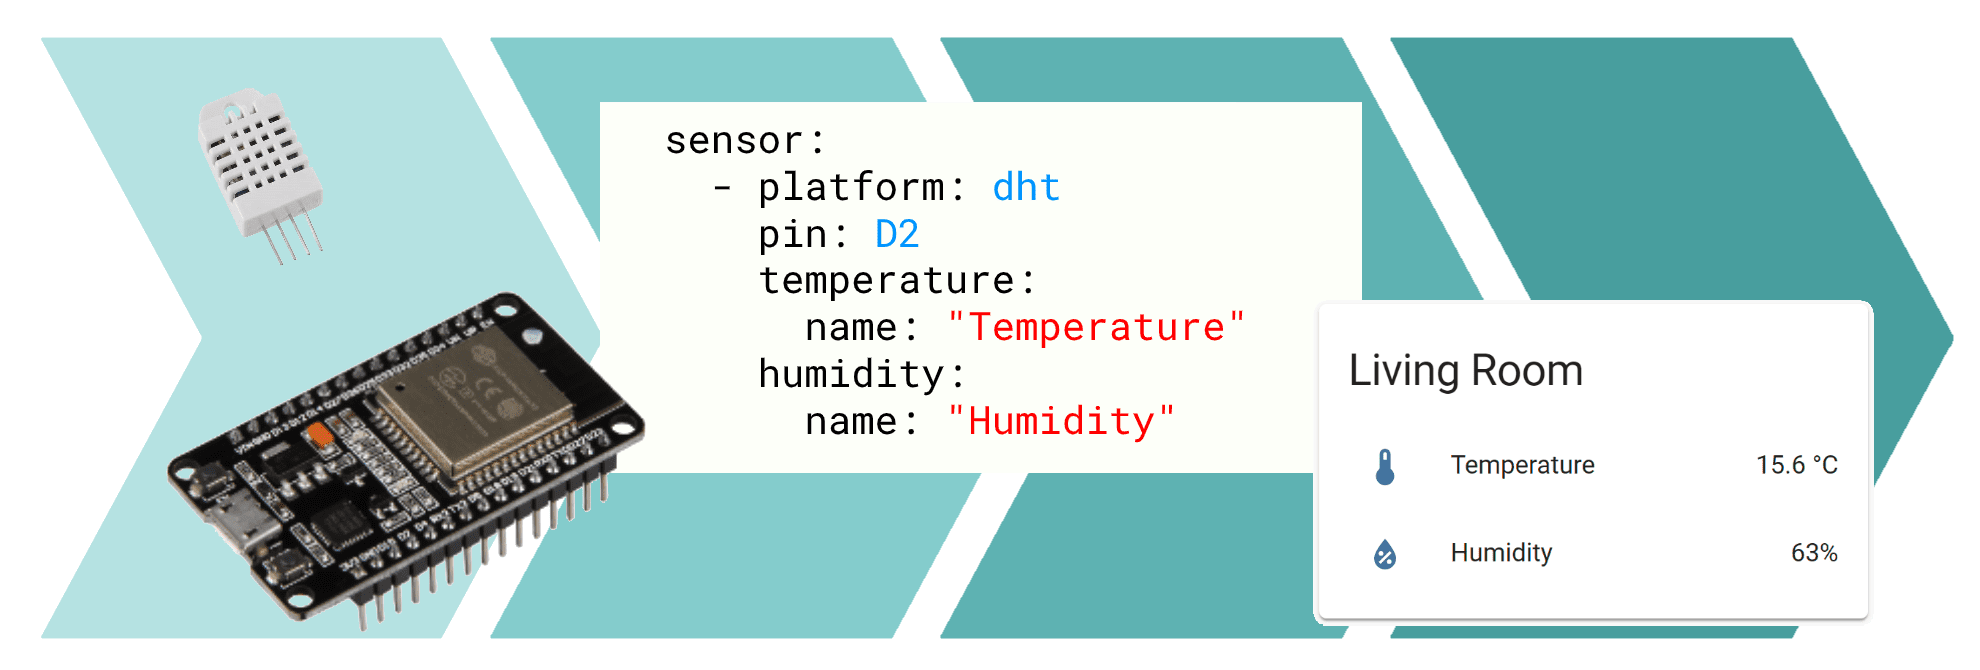
\includegraphics[width=0.45\paperwidth,keepaspectratio]{images/esp.png}
    \end{column}
  \end{columns}
\end{frame}

\subsection{Platforms}
% Platforms
\begin{frame}[fragile]
  \frametitle{Building Sensor Devices: The Controller}
  \begin{columns}[]
    \begin{column}[T]{0.45\paperwidth}
      ESPHome runs on easily obtained microcontroller hardware.
      \vfill
      Typical cost for an entire USB-powered sensor can be as low as \$5
      \begin{enumerate}%[<+->]
        \item{ESP32}
        \item{ESP8266}
        \item{Raspberry Pi RP2040 \tiny{(\emph{Slightly} easier finding one!)}}
      \end{enumerate}
    \end{column}
    \begin{column}[T]{0.45\paperwidth}
      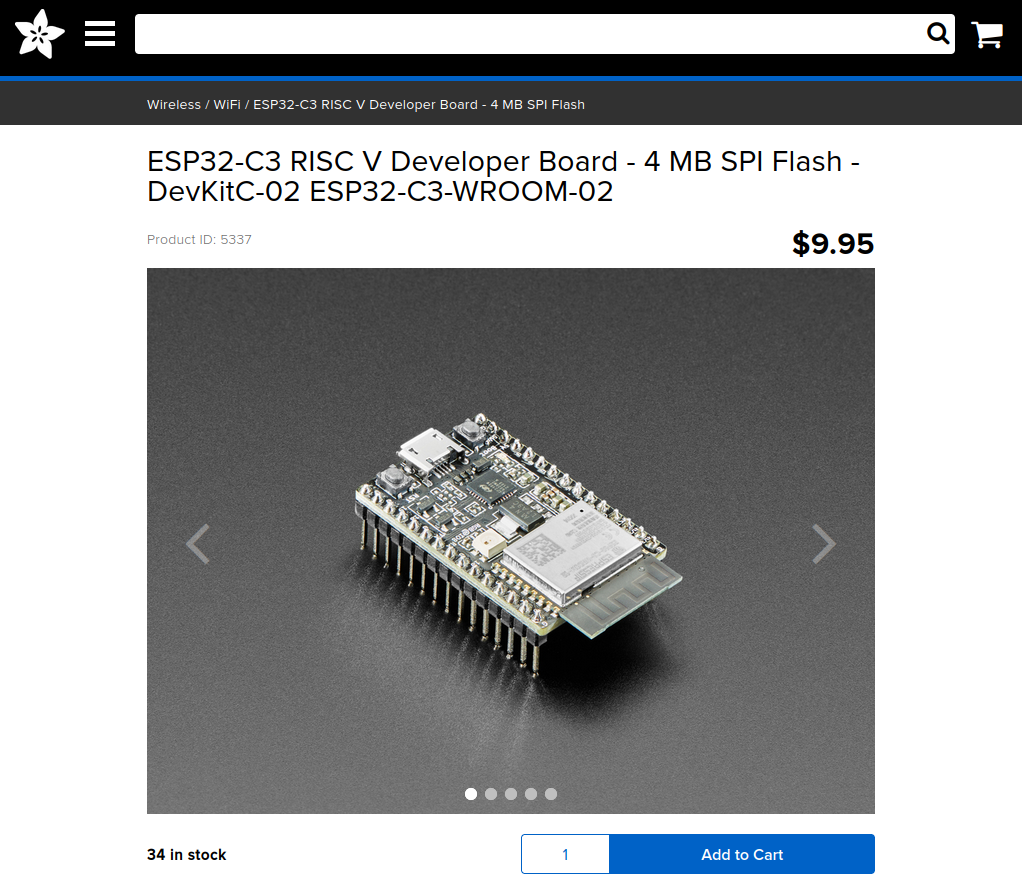
\includegraphics[width=0.45\paperwidth,keepaspectratio]{images/esp32-ada.png}
    \end{column}
  \end{columns}
\end{frame}

% Devices/Components
\subsection{Devices/Components}
\begin{frame}[fragile]
  \frametitle{Building Sensor Devices: The Sensors}
  \begin{columns}[]
    \begin{column}[T]{0.45\paperwidth}
      Types of common `sensor components':
      \begin{itemize}%[<+->]
        \item{Air Quality}
        \item{Digital Signals}
        \item{Distance}
        \item{Electricity/Power}
        \item{Environmental}
        \item{Light}
        \item{Magnetic}
        \item{Motion}
        \item{Weight}
      \end{itemize}
    \end{column}
    \begin{column}[T]{0.45\paperwidth}
      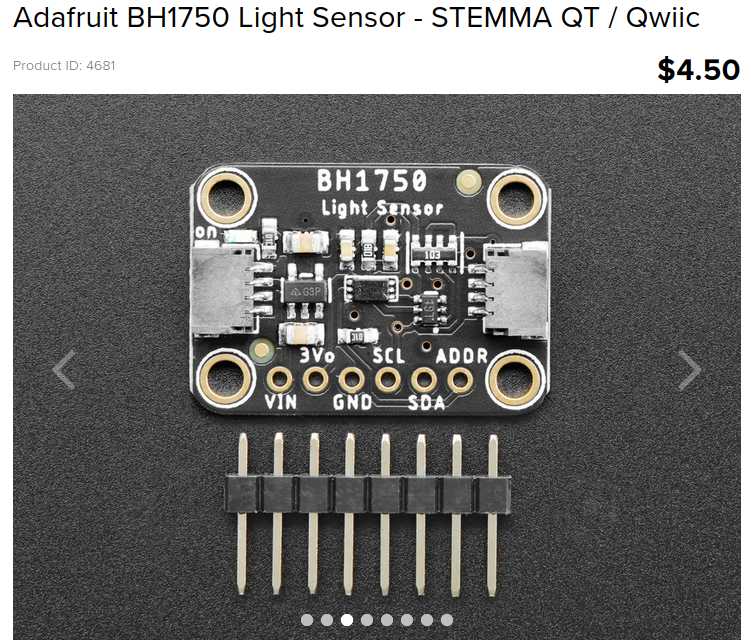
\includegraphics[width=0.45\paperwidth,keepaspectratio]{images/bh1750-ada.png}
    \end{column}
  \end{columns}
\end{frame}
% Configuration
\subsection{Configuration}
\begin{frame}[fragile]
  \frametitle{Building Sensor Devices: Putting It All Together}
  \begin{columns}[]
    \begin{column}[T]{0.45\paperwidth}
      A typical ESPHome config contains the following sections:
      \begin{enumerate}%[<+->]
        \item{Device name}
        \item{Board/Controller Definition}
        \item{WiFi Info}
        \item{Sensor Connection Setup}
        \item{Sensor Definition}
      \end{enumerate}
    \end{column}
    \begin{column}[T]{0.45\paperwidth}
      Example code configuring a custom light level sensor:
      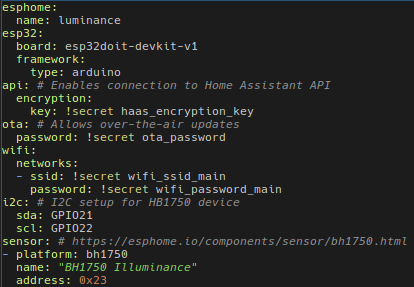
\includegraphics[width=0.45\paperwidth,keepaspectratio]{images/luminance.png}
    \end{column}
  \end{columns}
\end{frame}

\section{Usage and Demo (Part 2)}
% Demo of ESPHome
\subsection{Demo of ESPHome}
\frame{\subsectionpage}
\subsection{ESPHome devices in Home-Assistant}
\begin{frame}[fragile]
  \frametitle{Luminance Driven Light Switch}
  Home Assistant performs an Automation which does the following:
  \begin{enumerate}%[<+->]
    \item{Trigger}
      \begin{enumerate}
        \item{1.5 hours before the sun sets}
        \item{The time is 8am Eastern}
        \item{The BH1750 light sensor triggers an event}
      \end{enumerate}
    \item{Conditions}
      \begin{enumerate}
        \item{Time between 8am and 5pm Eastern, on a weekday}
        \item{The BH1750 sensor has been `dim' for 15 minutes}
        \item{My lamps are already off}
      \end{enumerate}
    \item{Actions}
      \begin{enumerate}
        \item{Turn on Office Table Lamp}
        \item{Turn on Desk Lamp}
      \end{enumerate}
  \end{enumerate}
\end{frame}

\section{Wrapping Up}
\frame{\sectionpage}

\begin{frame}
  \frametitle{Key Takeaways}
  \begin{itemize}[<+->]
    \item{Home Assistant is a pretty neat central, locally controlled, home automation system}
    \item{Creating your own sensors and doing useful things with them is very easy and inexpensive}
  \end{itemize}
\end{frame}

\begin{frame}[fragile]
  \frametitle{Issues and Lessons Learned}
  \begin{enumerate}
    \item{Great lessons in scripted updates}
    \item{Great use case for data analysis in Postgres}
    \item{Excellent lessons about bulk loading processes}
    \item{Even better lessons in tuning settings for regular large imports}
  \end{enumerate}
\end{frame}

\begin{frame}
  \frametitle{Thank You}
  \begin{center}
    \LARGE{Questions?}
    \vfill
    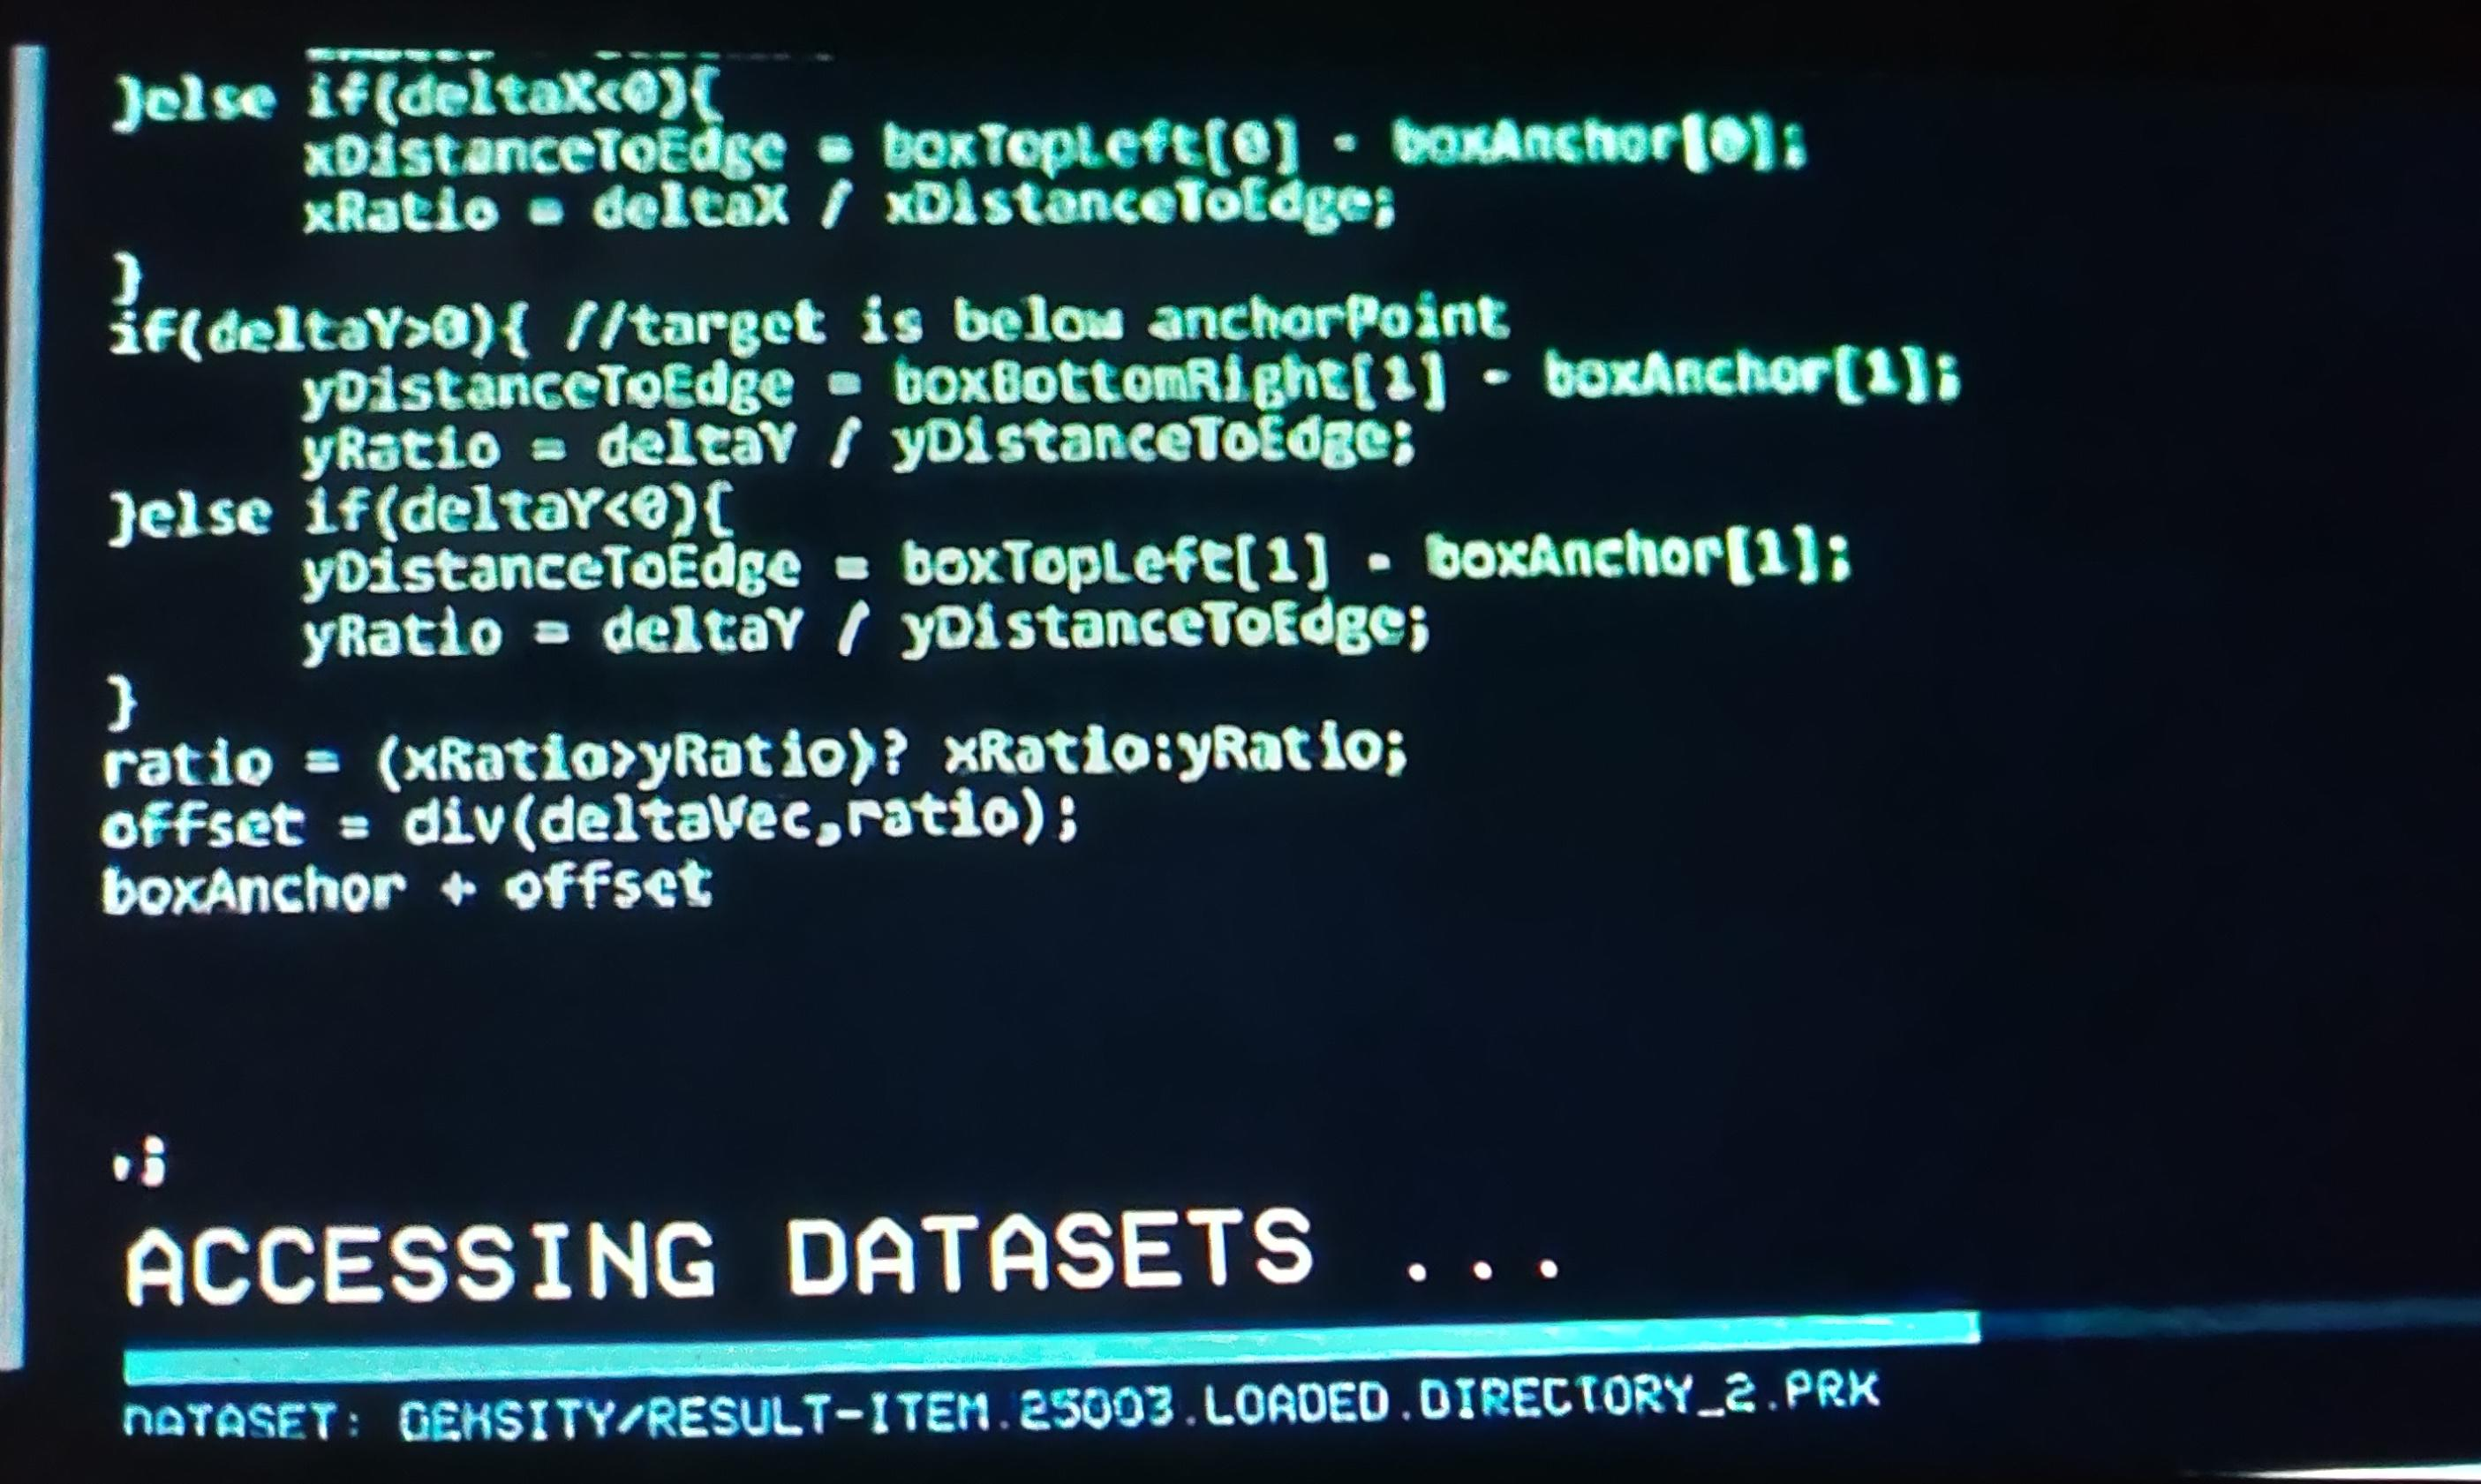
\includegraphics[height=5cm]{images/lol-code.jpg}
  \end{center}
\end{frame}
\begin{frame}[plain,fragile]
  \frametitle{References}
  \begin{columns}[]
    \begin{column}[T]{0.55\paperwidth}
      Code for this presentation, as well as some sample device manifests and other
      information can be found on GitHub and GitLab.
      \begin{itemize}
        \item{\href{https://github.com/tomswartz07/CPOSC2023}{https://github.com/tomswartz07/CPOSC2023}}
        \item{\href{https://gitlab.com/tom.swartz07/CPOSC2023}{https://gitlab.com/tom.swartz07/CPOSC2023}}
      \end{itemize}
      \vfill
      Further Reading:
      \begin{enumerate}
        \item{\href{https://www.home-assistant.io/}{https://www.home-assistant.io/}}
        \item{\href{https://esphome.io/}{https://esphome.io/}}
        \item{\href{https://www.troyhunt.com/iot-unravelled-part-1-its-a-mess-but-then-theres-home-assistant/}{https://www.troyhunt.com/ IoT Unravelled Series}}
      \end{enumerate}
    \end{column}
    \begin{column}[T]{0.35\paperwidth}
      \qrcode[height=1.5in]{https://github.com/tom.swartz07/CPOSC2023/}
    \end{column}
  \end{columns}
\end{frame}

\end{document}
% vim: set ts=2 sw=2 spell:
